\chap{Buttons/Switches}


\section{Objectives}
In this lab, you will
\begin{itemize}
    \item Learn how to use a timer and timer interrupt in STM32, and 
    \item Learn how to read digital inputs and display values to LEDs using a timer
\end{itemize}

\section{Introduction}
Embedded systems usually use button/switches as part of their user interface. This general rule applies from the most basic remote-control system for opening a garage door, right up to the most sophisticated aircraft autopilot system. Whatever the system you create, you need to be able to create a reliable button/switch interface. 

%add a picture of buttons/switch

In this lab, we consider how you read inputs from mechanical switches in your embedded application. 

Before considering button/switches themselves, we will consider the process of reading the state of port pins.

\section{Basic techniques for reading from port pins}

\subsection{The need for pull-up resistors}
\begin{figure}[!htp]
    \centering
    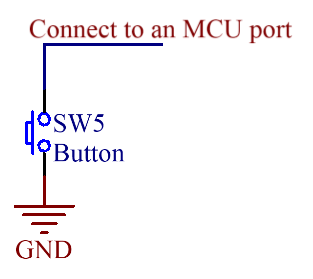
\includegraphics[width=2.5in]{source/picture/bai_4/Button_Schematic_0.png}
    \caption{\textit{Button/switch connects to an MCU}}
    \label{bai4_pic_button_schematic_0}
\end{figure}
Figure \ref{bai4_pic_button_schematic_0} shows a normal way to connect a button/switch to an MCU. This hardware operates as follows:
\begin{itemize}
    \item When the switch is open, it has no impact on the port pin. An internal resistor on the port ``pulls up" the pin to the supply voltage of the microcontroller (typically 3.3V for STM32F103). If we read the pin, we will see the value `1'. 
    \item When the switch is closed (pressed), the pin voltage will be 0V. If we read the pin, we will see the value `0'. 
\end{itemize}
 
 However, if the MCU does not have a pull-up resistor inside, when the button is pressed, the read value will be `0', but even we release the button, the read value is still `0' as shown in Figure \ref{bai4_pic_the_need_of_pull_up_resistors}.
 \begin{figure}[!htp]
    \centering
    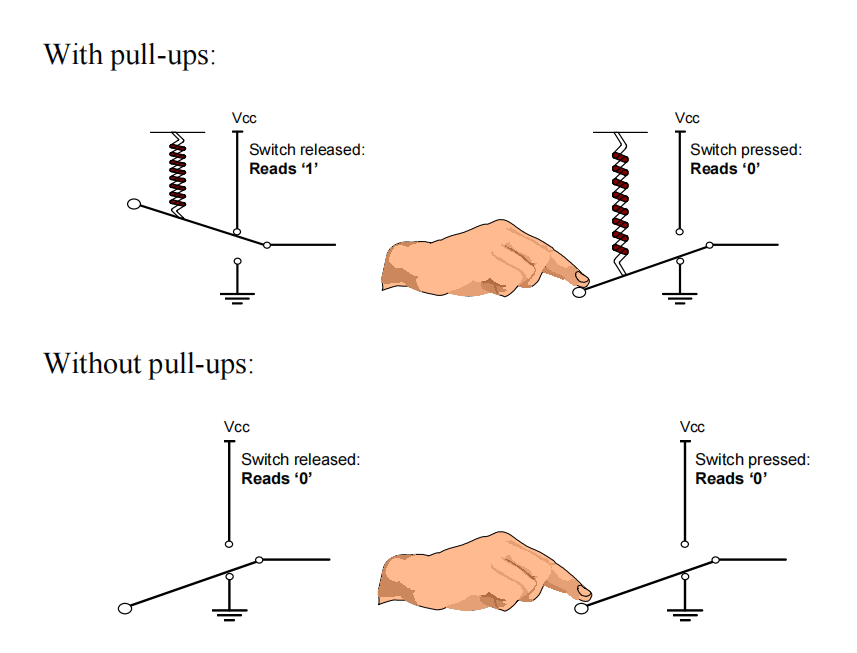
\includegraphics[width=5.5in]{source/picture/bai_4/pullup_resistors.png}
    \caption{\textit{The need of pull up resistors}}
    \label{bai4_pic_the_need_of_pull_up_resistors}
\end{figure}
%add a picture 

So a reliable way to connect a button/switch to an MCU is that we explicitly use an external pull-up resistor as shown in Figure \ref{bai4_pic_button_schematic_1}.

 \begin{figure}[!htp]
    \centering
    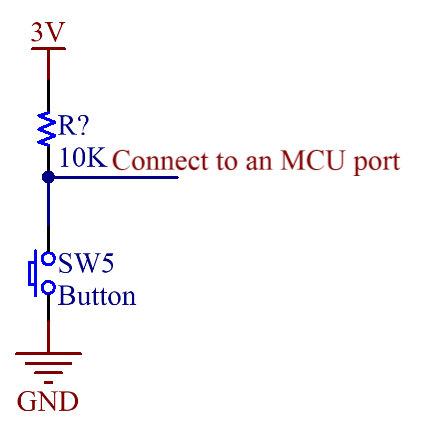
\includegraphics[width=2in]{source/picture/bai_4/Button_Schematic.png}
    \caption{\textit{A reliable way to connect a button to an MCU}}
    \label{bai4_pic_button_schematic_1}
\end{figure}
 
 
\subsection{Dealing with switch bounce}
In practice, all mechanical switch contacts bounce (that is, turn on and off, repeatedly, for short period of time) after the switch is closed or opened as shown in Figure \ref{bai4_pic_switchsbounce}.

As far as the MCU concerns, each “bounce” is equivalent to one press and release of an “ideal” switch. 
Without appropriate software design, this can give several problems:
\begin{itemize}
    \item Rather than reading ‘A’ from a keypad, we may read ‘AAAAA’
    \item Counting the number of times that a switch is pressed becomes extremely difficult
    \item If a switch is depressed once, and then released some time later, the 'bounce' may make it appear as if the switch has been pressed again (at the time of release). 
\end{itemize}
\begin{figure}[!htp]
    \centering
    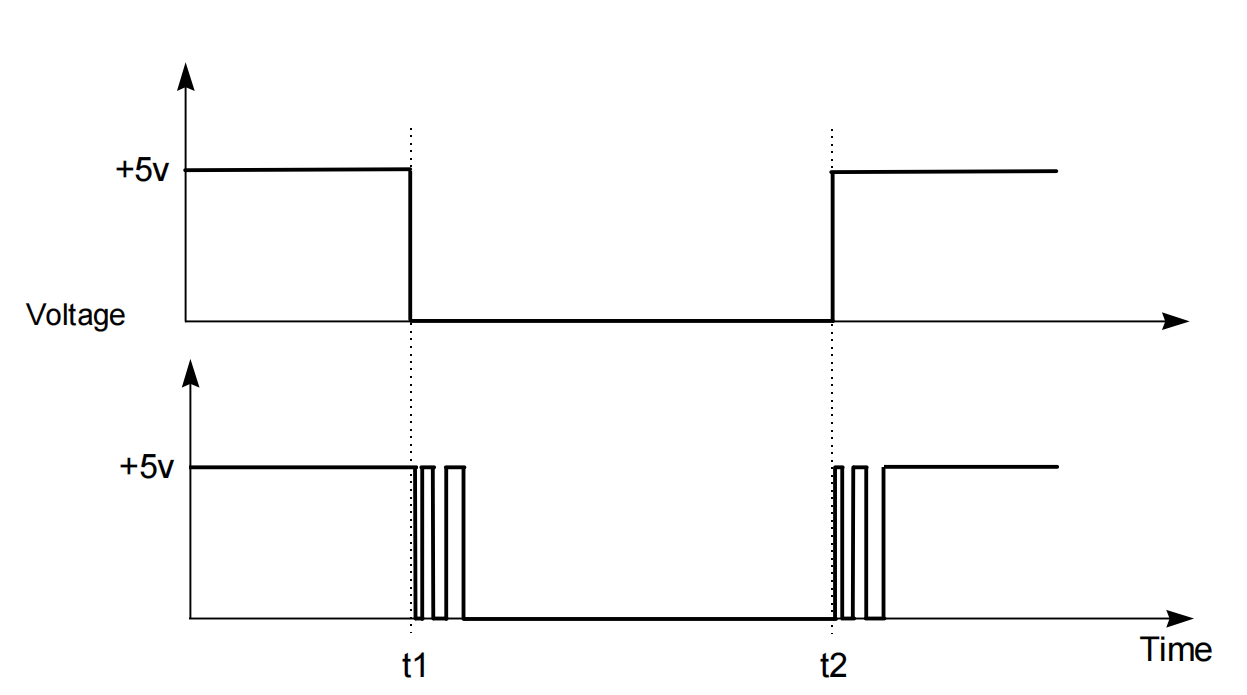
\includegraphics[width=5.5in]{source/picture/bai_4/switchsbounce.png}
    \caption{\textit{Switch bounces}}
    \label{bai4_pic_switchsbounce}
\end{figure}


Creating a simple software to check for a valid switch input is straightforward:
\begin{itemize}
    \item Read the relevant port pin
    \item If we think we have detected a switch depression, we wait for 20ms and then read the pin again.
    \item If the second reading confirms the first reading, we assume the switch really has been depressed.
\end{itemize}

Note that the figure of ‘20ms’ will depend on the switch used and the deployed environment. 

\section{Reading switch inputs (basic code) using STM32}
This switch reading code is adequate if we want to perform operations such as:
\begin{itemize}
    \item Drive a motor while a switch is pressed.
    \item Swith on a light while a switch is pressed.
    \item Activate a pump while a switch is pressed.
\end{itemize}
These operations could be implemented using an electrical switch without using a microcontroller; however, use of a microcontroller may well be appropriate if we require more complex behaviour. For example:
\begin{itemize}
    \item Drive a motor while a switch is pressed. 
    
    Condition: If the safety guard is not in place, don't turn the motor. Instead sound a buzzer for 2 seconds. 
    \item Swith on a light while a switch is pressed.
    
    Condition: To save power, ignore requests to turn on the light during daylight hours. 
    
    \item Activate a pump while a switch is pressed
    
    Condition: If the main water reservoir is below 300 litres, do not start the main pump: instead, start the reserve pump and draw teh water from the emergency tank. 
\end{itemize}
\subsection{Setting up}
\subsubsection{Create a project}
Please follow the instruction in Labs 1 and 2 to create a project that includes: 
\begin{itemize}
    \item PB0 as an input port pin as shown in Figure \ref{bai4_pic_input_output_setting}, 
    \item PA0-PA7 as output port pins as shown in Figure \ref{bai4_pic_input_output_setting}
    \item Timer 2 10ms interrupt
\end{itemize}

\begin{figure}[!htp]
    \centering
    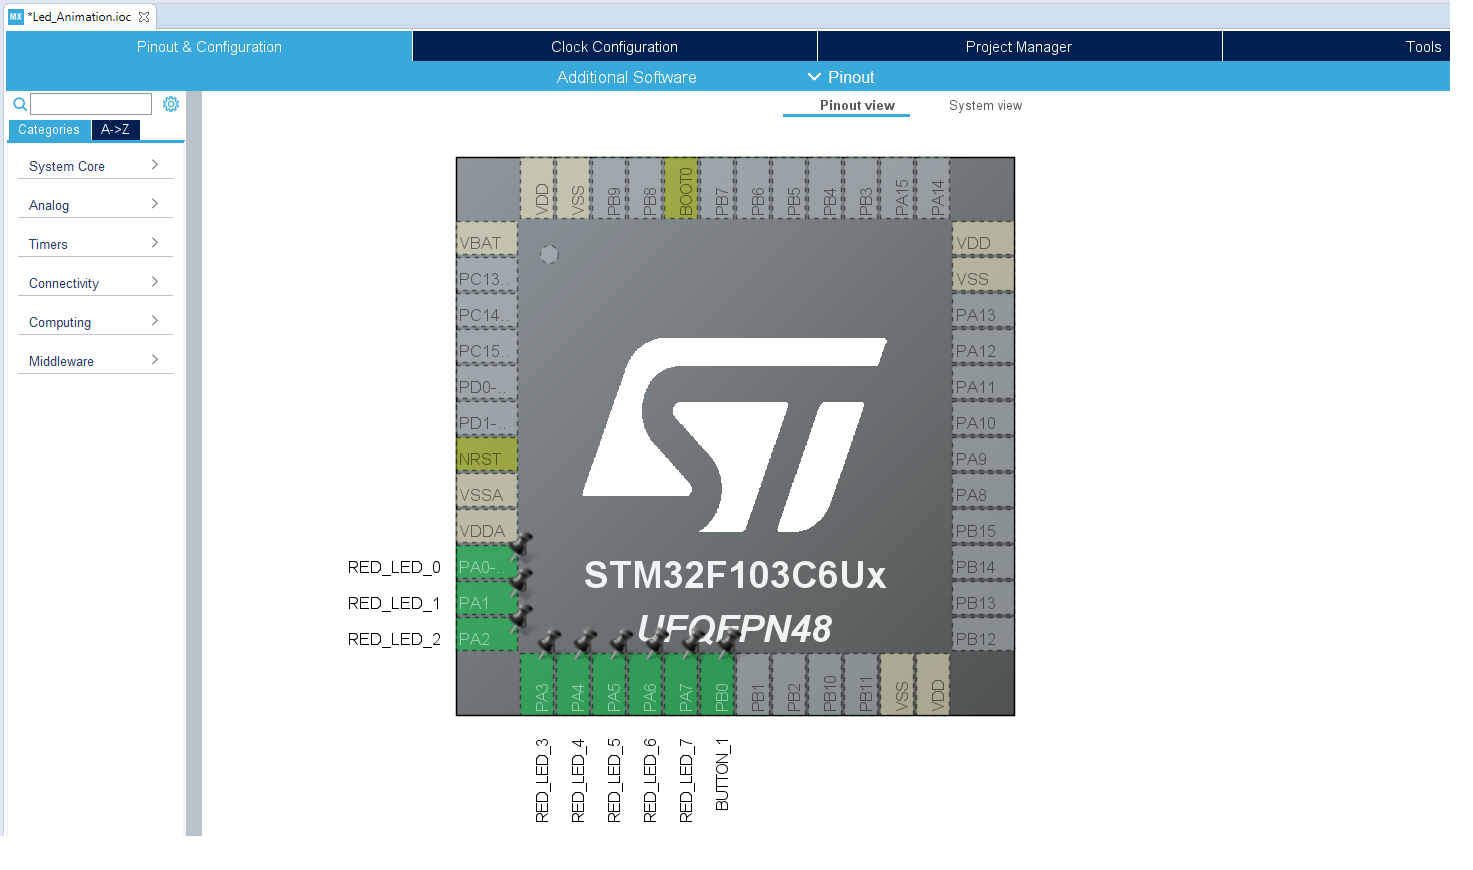
\includegraphics[width=5.5in]{source/picture/bai_4/Input_Output_Settings.png}
    \caption{\textit{Input Output Setting}}
    \label{bai4_pic_input_output_setting}
\end{figure}

\subsubsection{Input Output Processing Patterns}
For both input and output processing, we have a similar pattern to work with. Normally, we have a module named driver which works directly to the hardware. We also have a buffer to store temporarily values. In the case of input processing, the driver will store the value of the hardware status to the buffer for further processing. In the case of output processing, the driver uses the buffer data to output to the hardware. 

\begin{figure}[!htp]
    \centering
    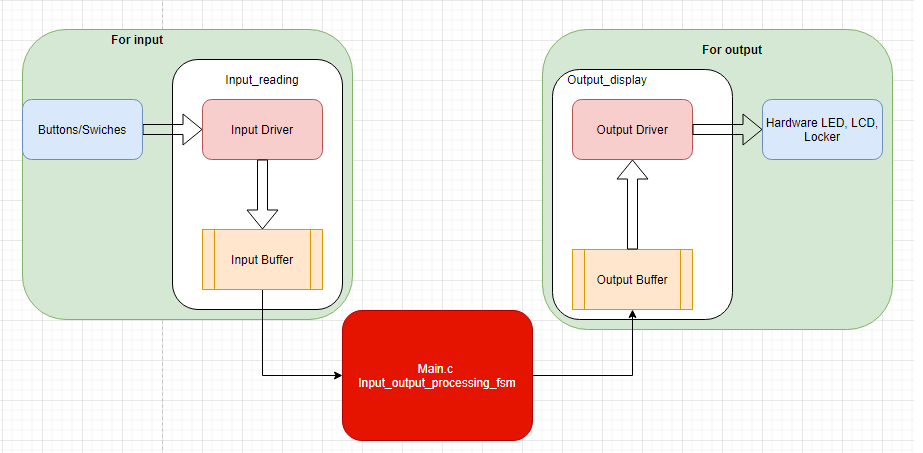
\includegraphics[width=5.5in]{source/picture/bai_4/Input_Output_patterns.png}
    \caption{\textit{Input Output Processing Patterns}}
    \label{bai4_pic_Input_Output_patterns}
\end{figure}

Figure \ref{bai4_pic_Input_Output_patterns} shows that we should have an input\_reading module to processing the buttons, then store the processed data to the buffer. Then a module of input\_output\_processing\_fsm will process the input data, and update the output buffer. The output driver gets the value from the output buffer to transfer to the hardware. 

\subsubsection{Create a file C source file and header file for input reading}

\begin{figure}[!htp]
    \centering
    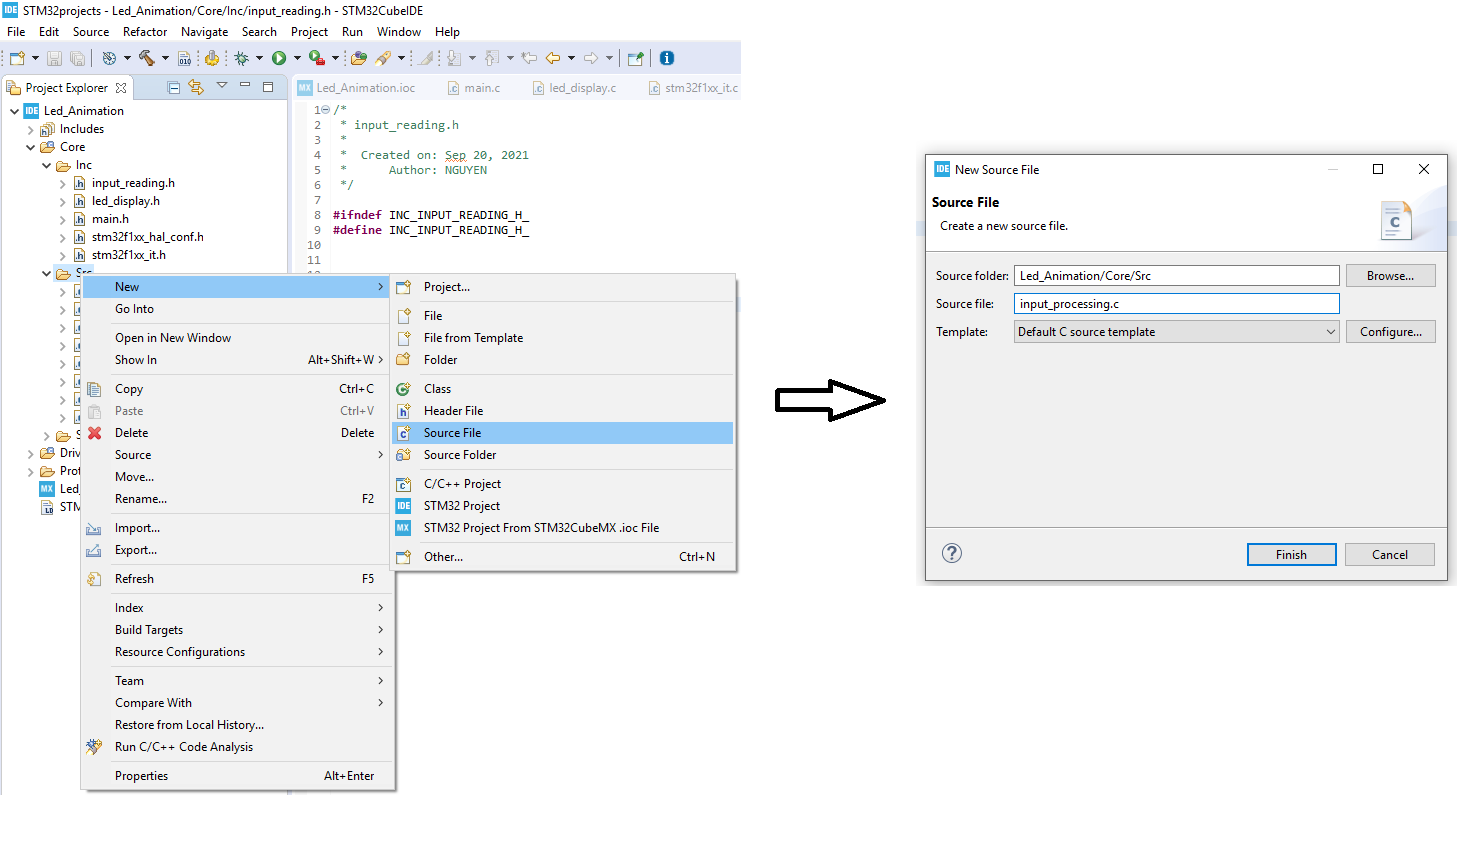
\includegraphics[width=5.5in]{source/picture/bai_4/Adding_new_files_to_project_step_1.png}
    \caption{\textit{Step 1: Create a C source file for input reading}}
    \label{bai4_pic_Adding_new_files_to_project_step_1}
\end{figure}

\begin{figure}[!htp]
    \centering
    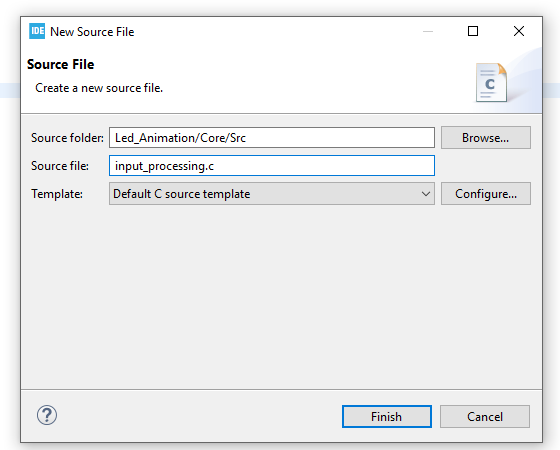
\includegraphics[width=5.5in]{source/picture/bai_4/Adding_new_files_to_project_step_2.png}
    \caption{\textit{Step 2: Create a C header file for input reading}}
    \label{bai4_pic_Adding_new_files_to_project_step_2}
\end{figure}

\begin{figure}[!htp]
    \centering
    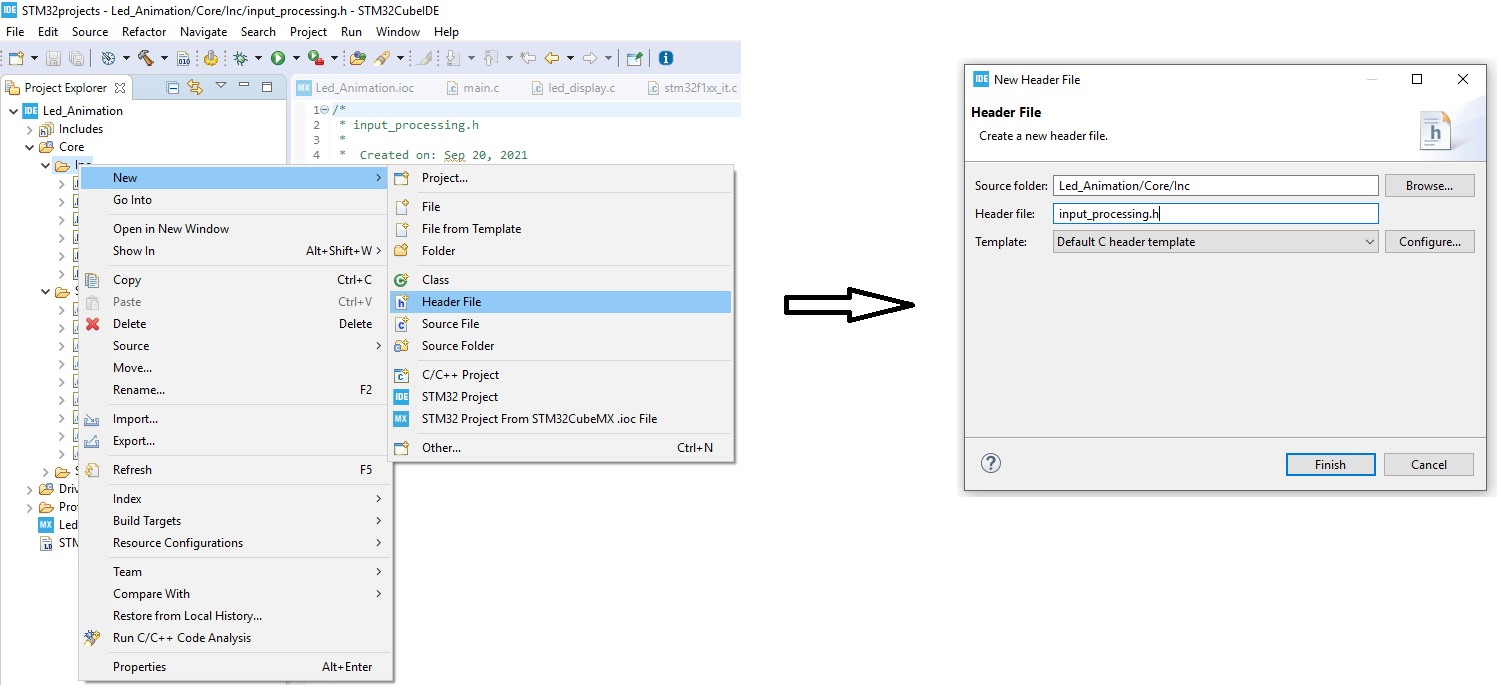
\includegraphics[width=5.5in]{source/picture/bai_4/Adding_new_files_to_project_step_3.png}
    \caption{\textit{Step 3: Create a C source file for input processing}}
    \label{bai4_pic_Adding_new_files_to_project_step_3}
\end{figure}

\begin{figure}[!htp]
    \centering
    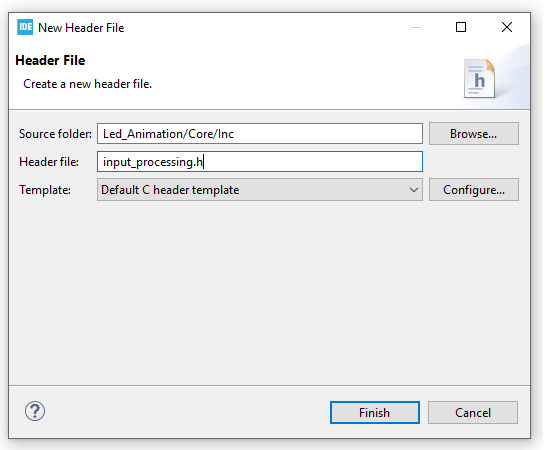
\includegraphics[width=5.5in]{source/picture/bai_4/Adding_new_files_to_project_step_4.png}
    \caption{\textit{Step 4: Create a C header file for input processing}}
    \label{bai4_pic_Adding_new_files_to_project_step_4}
\end{figure}

\begin{figure}[!htp]
    \centering
    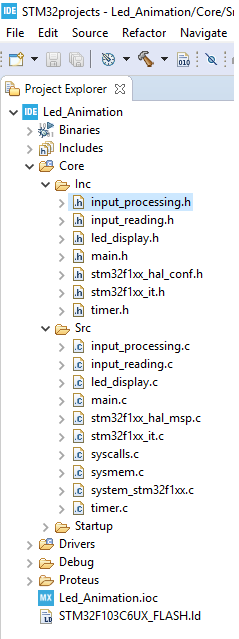
\includegraphics[width=5.5in]{source/picture/bai_4/Adding_new_files_to_project.png}
    \caption{\textit{Input Output Setting}}
    \label{bai4_pic_Adding_new_files_to_project}
\end{figure}


\subsection{How to read Port Pin}

\section{Problem 1}

In this week lab, assume you have two button and 8 LEDs, you have to write a program that
\begin{itemize}
    \item Has a timer which has an interrupt in every 10 milliseconds.  
    \item  Reads values of buttons 1 and 2 every 10 milliseconds. The read button function should be called inside the timer interrupt service routine.
    \item Increases the value of LEDs connected to PORTC when the button 1 is pressed.
    \item Increases the value of PORTC automatically in every 0.5 second, if the button 1 is pressed in more than 1 second.
    \item Increases the value of PORTC automatically in every 0.1 second, if the button 1 is pressed in more than 3 seconds.
    \item Decreases the value of PORTC when the button 2 is pressed
    \item Decreases the value of PORTC automatically in every 0.5 second, if the button 2 is pressed in more than 1 second.
    \item Decreases the value of PORTC automatically in every 0.1 second, if the button 2 is pressed in more than 3 seconds.
    \item The above values such as 10 ms, 0.5 s, 0.1s, 1 s and 3 s are fixed values as an example. Your program, however, needs to provide an easy way to change those values. For example, you should use DEFINE to define those values.
    \item If both buttons 1 and 2 are pressed, button 1 has a higher priority.
\end{itemize}


\section{Problem 2 - A digital clock}
 You have to write a program that mimics a Casio digital watch. Assume you have 2 buttons and 6 seven-segment LED, a program should have
\begin{itemize}
    \item A normal clock that shows hours, minutes, and seconds on 6 seven-segment LEDs.
    \item  A stopwatch that shows minutes, seconds and 1/100 second
    \item We use button 1 to change modes of a digital watch. Every time button 1 is pressed, the watch will change to the next mode.
    \item Mode 0: runs normal clock (default)
    \item Mode 1: modifies hours. In this mode, the hour number is blinking, and button 2 is used for increasing the hour number.  If button 2 is kept pressed more than 1 second, the hour number will increase automatically, i.e., 5 times per second. Please note that the hour number should be returned to 0 when it reaches 23.
    \item  Mode 2: modifies minutes. Similar to mode 1, the minute number is blinking and increases when button 2 is pressed.
    \item Mode 3: modifies seconds. Similar to mode 1, the second number is blinking and increases when button 2 is pressed.
    \item Mode 4: runs a stopwatch. Using button 2 to start and stop the watch.  
 
\end{itemize}
 Please note that while the stopwatch is running, the normal clock is still running in the background.


 

\section{Instructions}

Your task is to sketch an FSM that describes your idea of how to solve the above problem and  writes a firmware that runs on STM32.



 

\section{Submission}

You need to
\begin{itemize}
    \item Demonstrate your work in the lab class and then
    \item  Submit your FSM sketches and source code to the BKeL.
\end{itemize}
